\section{Implementation}

\subsection{Implementation}
\begin{frame}
	\frametitle{Implementation}
	\begin{itemize}
		\setlength\itemsep{1em}
		\item All algorithms were implemented in C++, 
			using OpenMP for multithreading.
		\item Use the compressed sparse row (CSR) representation 
			for graph storage.
		\item To avoid modifying the graph, we have a boolean
			array termed \textit{valid} which signifies if a vertex is yet to be
			placed in an SCC.
	\end{itemize}
\end{frame}

\subsection{Trim Step}
\begin{frame}
	\frametitle{Trim Step}
	\begin{itemize}
		\setlength\itemsep{1em}
		\item It requires a single pass through all vertices to find 
			their in/out degrees, and flip their \textit{valid} boolean 
			if either degree is zero.
		\item To avoid the synchronization overhead, we maintain separate 
			queues for each thread, and combine them into the next level queue
			at the end of each iteration.
	\end{itemize}
\end{frame}

\subsection{Breath-First Search}
\begin{frame}
	\frametitle{Breath-First Search}
	\begin{itemize}
		\setlength\itemsep{1em}
		\item Using thread-local queues instead of a shared queue avoids the 
			synchronization overhead of insertions.
		\item A boolean \textit{visited} array outerperforms a bitmap.
		\item In this \textit{direction-optimizing} approach to BFS, all
			unvisited vertices attempt to find a parent that is in the 
			frontier, instead of the typical way of inspecting adjacencies of
			frontier vertices.
	\end{itemize}
\end{frame}

\subsection{Coloring}
\begin{frame}
	\frametitle{Coloring}
	\begin{itemize}
		\item Place the parent in queue to avoid explicit locking.
	\end{itemize}
	\begin{figure}
		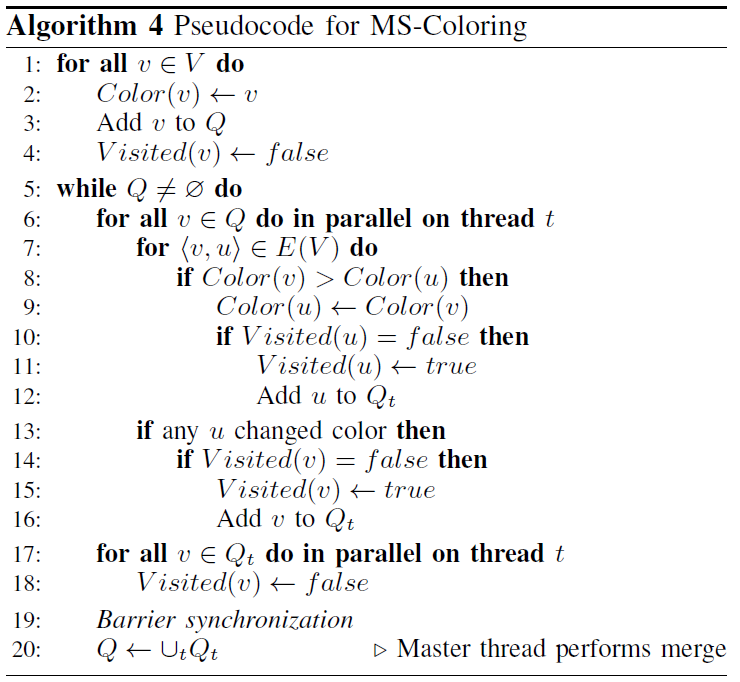
\includegraphics[scale=0.30]{figure/fig-MS-coloring.png}
	\end{figure}
\end{frame}

\subsection{BiCC Decomposition}
\begin{frame}
	\frametitle{BiCC Decomposition}
	\begin{itemize}
		\setlength\itemsep{1em}
		\item A new parallel approach for BiCC decomposition by identifying 
			articulation vertices in graph.
		\item An articulation vertex $u$ can be identified by the fact that it 
			has at least one child vertex that does not have a simple path in
			$G(V \setminus \{u\}, E(V \setminus \{u\})))$ to another vertex with 
			the same BFS level as $u$.
	\end{itemize}
\end{frame}

\begin{frame}
	\begin{figure}
		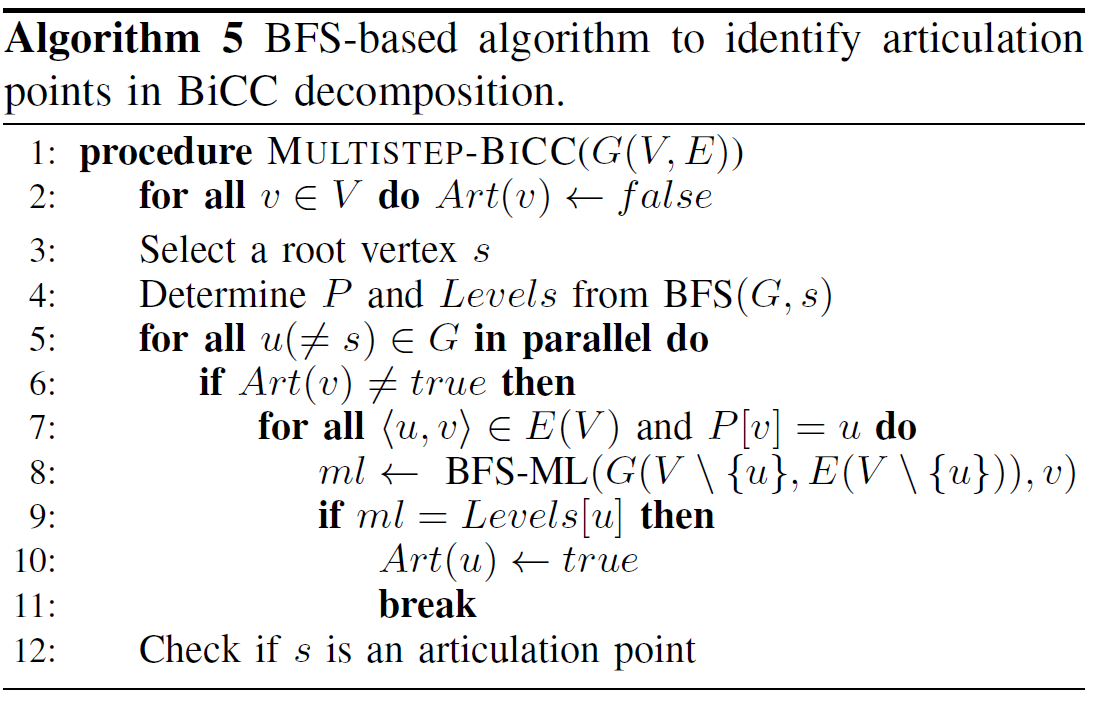
\includegraphics[scale=0.25]{figure/fig-BBC-BFS-based.png}
	\end{figure}
\end{frame}